\documentclass[12pt]{article}
\usepackage{amsmath,amssymb}
\usepackage{physics}
\usepackage{geometry}
\geometry{margin=1in}
\usepackage{tikz}
\usetikzlibrary{
    arrows.meta,
    calc,
    angles,
    quotes,
    decorations.pathmorphing
}
\usepackage[american]{circuitikz}


\begin{document}

\begin{center}
\Large \textbf{Advanced Integrated Physics Problem Set -- IV (Ultra-Hard Elite Version)}\\
\large 15 Deep Multi-Stage, Lengthy, Single-Correct Problems
\end{center}

\bigskip

%%%%%%%%%%%%%%%%%%%%%%%%%%%%%%%%%%%%%%%%%%%%%%%%%%%%%%%%%%%%
\textbf{Q1. Bead on Rotating Parabolic Wire in Axial Magnetic Field}


A smooth rigid wire is bent to form the curve $z = a r^2$ in cylindrical coordinates and is fixed in space. The entire system rotates with constant angular velocity $\omega$ about the vertical $z$-axis. A bead of mass $m$ and charge $q$ is constrained to move frictionlessly along the wire. A uniform magnetic field $\vec B = B\hat z$ fills all space.

Working in the rotating frame and carefully projecting Lorentz force along the tangent direction (not radially), determine the exact equilibrium condition for non-zero radius $r_0$, accounting for centrifugal, gravitational, and magnetic contributions.

\begin{center}
\begin{tikzpicture}[scale=1.1]

% Axes
\draw[->] (0,0) -- (0,4) node[above] {$z$};
\draw[->] (0,0) -- (4,0) node[right] {$r$};

% Parabolic curve
\draw[thick,domain=0:2,samples=100] plot (\x,{0.5*\x*\x});

% Bead
\fill (1.4,{0.5*1.4*1.4}) circle (2pt);
\node[right] at (1.4,{0.5*1.4*1.4}) {$m,q$};

% Magnetic field arrow
\draw[->,thick] (3.5,2) -- (3.5,3);
\node at (3.5,3.3) {$\vec B$};

% Rotation about z-axis
\draw[->] (0.6,3.2) arc (0:300:0.6);
\node at (1.2,3.8) {$\omega$};

\end{tikzpicture}
\end{center}

\begin{enumerate}
\item[(A)] $2agr_0 = \omega^2 r_0 - \dfrac{qB\omega}{m} r_0$
\item[(B)] $2agr_0 = \omega^2 r_0 + \dfrac{qB\omega}{m} r_0$
\item[(C)] $2agr_0 = \omega^2 r_0$
\item[(D)] $2agr_0 = \omega^2 r_0 - \dfrac{2qB\omega}{m} r_0$
\end{enumerate}

%%%%%%%%%%%%%%%%%%%%%%%%%%%%%%%%%%%%%%%%%%%%%%%%%%%%%%%%%%%%
\textbf{Q2. Block–Spring–Wedge with Moving Constraint and Internal Coupling}



A wedge of mass $M$ rests on a frictionless horizontal surface. A block of mass $m$ rests on the incline of angle $\theta$ and is connected to a fixed vertical wall via a spring of stiffness $k$. All surfaces are smooth. After release, the wedge is free to move horizontally.

Using a non-inertial description in the wedge frame and eliminating the constraint force via horizontal momentum conservation, determine the small oscillation frequency of the block relative to the wedge equilibrium.

\begin{center}
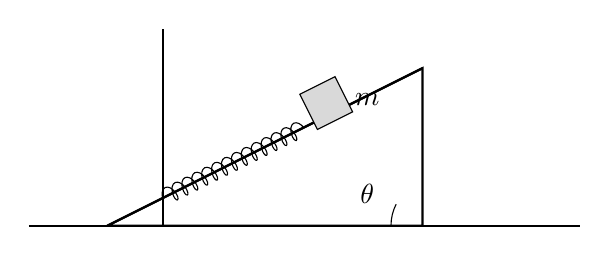
\begin{tikzpicture}[scale=1]

% Ground
\draw[thick] (-1,0) -- (6,0);

% Wedge (proper triangle)
\draw[thick] (0,0) -- (4,0) -- (4,2) -- cycle;

% Inclined surface explicitly drawn
\draw[thick] (0,0) -- (4,2);

% Block aligned on incline
\begin{scope}[rotate around={26.565:(2.8,1.4)}]
\draw[fill=gray!30] (2.6,1.3) rectangle (3.1,1.8);
\end{scope}
\node at (3.3,1.6) {$m$};

% Spring along incline
\draw[decorate,decoration={coil,aspect=0.5,segment length=4pt,amplitude=3pt}]
(0.7,0.35) -- (2.6,1.3);

% Wall
\draw[thick] (0.7,0) -- (0.7,2.5);

% Angle theta
\draw (3.6,0) arc (180:153:0.6);
\node at (3.3,0.4) {$\theta$};

\end{tikzpicture}
\end{center}
\begin{enumerate}
\item[(A)] $\sqrt{\dfrac{k(M+m)}{mM}}$
\item[(B)] $\sqrt{\dfrac{k(M+m\sin^2\theta)}{mM}}$
\item[(C)] $\sqrt{\dfrac{k}{m} \cdot \dfrac{M+m}{M+m\sin^2\theta}}$
\item[(D)] $\sqrt{\dfrac{k}{m} \cdot \dfrac{M+m\sin^2\theta}{M+m}}$
\end{enumerate}

%%%%%%%%%%%%%%%%%%%%%%%%%%%%%%%%%%%%%%%%%%%%%%%%%%%%%%%%%%%%
\textbf{Q3. Coulomb Orbit in Weak Uniform Electric Field (Shifted Central Orbit)}

A particle of mass $m$ and charge $q$ moves under Coulomb attraction of a fixed charge $Q$ at the origin. A weak uniform electric field $E$ acts along the $+x$-direction. Treating the field as a perturbation and expanding the effective potential to first order in $E$, determine the leading-order shift in the circular orbit radius $r_0$.

\begin{enumerate}
\item[(A)] $\dfrac{qE r_0^3}{kQq}$
\item[(B)] $\dfrac{E r_0^3}{kQ}$
\item[(C)] $\dfrac{E r_0^2}{kQ}$
\item[(D)] $\dfrac{qE r_0^2}{kQq}$
\end{enumerate}

%%%%%%%%%%%%%%%%%%%%%%%%%%%%%%%%%%%%%%%%%%%%%%%%%%%%%%%%%%%%
\textbf{Q4. Rotating Conducting Rod in Uniform Magnetic Field}



A conducting rod of length $L$ rotates with constant angular velocity $\omega$ about one fixed end in a region of uniform magnetic field $\vec B = B\hat z$. The rod lies in the horizontal plane. Charge redistribution occurs due to motional emf.

Using differential emf integration $d\mathcal{E} = ( \vec v \times \vec B )\cdot d\vec l$, determine the potential difference between the free end and pivot.

\begin{center}
\begin{tikzpicture}[scale=1]

% Pivot
\fill (0,0) circle (2pt);

% Rod
\draw[thick] (0,0) -- (4,0);
\node[below] at (2,0) {$L$};

% Magnetic field into page
\node at (4.5,0.5) {$\otimes B$};

% Angular velocity
\draw[->] (1.5,0.6) arc (20:80:0.8);
\node at (1.5,1.5) {$\omega$};

\end{tikzpicture}
\end{center}

\begin{enumerate}
\item[(A)] $\dfrac{1}{2} B\omega L^2$
\item[(B)] $B\omega L^2$
\item[(C)] $\dfrac{1}{3} B\omega L^2$
\item[(D)] $\dfrac{2}{3} B\omega L^2$
\end{enumerate}

%%%%%%%%%%%%%%%%%%%%%%%%%%%%%%%%%%%%%%%%%%%%%%%%%%%%%%%%%%%%
\textbf{Q5. Circular Satellite Orbit with Weak Quadratic Drag}

A satellite of mass $m$ moves initially in a circular orbit of radius $r_0$ around Earth. A weak resistive force proportional to $v^2$, $F = -\beta v^2$, acts opposite velocity. Assuming the orbit remains nearly circular over one revolution, compute the fractional change in radius per revolution using orbital energy decay.

\begin{enumerate}
\item[(A)] $-\dfrac{2\pi \beta r_0}{m}$
\item[(B)] $-\dfrac{4\pi \beta r_0}{m}$
\item[(C)] $-\dfrac{2\pi \beta r_0^2}{m}$
\item[(D)] $-\dfrac{\pi \beta r_0}{m}$
\end{enumerate}

%%%%%%%%%%%%%%%%%%%%%%%%%%%%%%%%%%%%%%%%%%%%%%%%%%%%%%%%%%%%
\textbf{Q6. Bead on Inclined Rotating Rod}


A straight smooth rod makes angle $\alpha$ with the vertical and rotates with constant angular velocity $\omega$ about the vertical axis passing through its lower end. A bead of mass $m$ can slide without friction along the rod.

Derive the equilibrium condition by balancing gravitational and centrifugal components projected along the rod.

\begin{center}
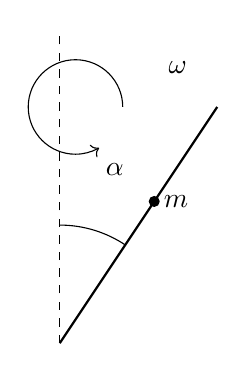
\begin{tikzpicture}[scale=1]

% Vertical axis
\draw[dashed] (0,0) -- (0,4);

% Rod
\draw[thick] (0,0) -- (2,3);

% Angle alpha
\draw (0,1.5) arc (90:56:1.5);
\node at (0.7,2.2) {$\alpha$};

% Bead
\fill (1.2,1.8) circle (2pt);
\node[right] at (1.2,1.8) {$m$};

% Rotation about vertical axis
\draw[->] (0.8,3) arc (0:300:0.6);
\node at (1.5,3.5) {$\omega$};

\end{tikzpicture}
\end{center}

\begin{enumerate}
\item[(A)] $mg\cos\alpha = m\omega^2 s\sin\alpha$
\item[(B)] $mg\sin\alpha = m\omega^2 s\sin\alpha$
\item[(C)] $mg\cos\alpha = m\omega^2 s$
\item[(D)] $mg = m\omega^2 s\sin\alpha$
\end{enumerate}

%%%%%%%%%%%%%%%%%%%%%%%%%%%%%%%%%%%%%%%%%%%%%%%%%%%%%%%%%%%%
\textbf{Q7. Radial Oscillation in $1/r + 1/r^3$ Potential}

A particle moves in potential
\[
U(r)= -\frac{k}{r} + \frac{\gamma}{r^3}
\]
where $\gamma \ll kr_0^2$. For a stable circular orbit at $r_0$, small radial oscillations occur. Determine the radial oscillation frequency by evaluating the second derivative of effective potential.

\begin{enumerate}
\item[(A)] $\sqrt{\dfrac{k}{mr_0^3} - \dfrac{6\gamma}{mr_0^5}}$
\item[(B)] $\sqrt{\dfrac{k}{mr_0^3} + \dfrac{6\gamma}{mr_0^5}}$
\item[(C)] $\sqrt{\dfrac{3k}{mr_0^3} - \dfrac{2\gamma}{mr_0^5}}$
\item[(D)] $\sqrt{\dfrac{3k}{mr_0^3} + \dfrac{2\gamma}{mr_0^5}}$
\end{enumerate}

%%%%%%%%%%%%%%%%%%%%%%%%%%%%%%%%%%%%%%%%%%%%%%%%%%%%%%%%%%%%
\textbf{Q8. Dielectric Slab in Isolated Capacitor with Mechanical Coupling}


A parallel-plate capacitor with variable capacitance $C(x)$ is charged and then disconnected from the battery. A dielectric slab of mass $m$ partially inserted is attached to a spring of constant $k$. The charge on plates remains constant.

Using total energy $U = \dfrac{Q^2}{2C(x)} + \dfrac12 kx^2$, determine the small oscillation frequency about equilibrium.

\begin{center}
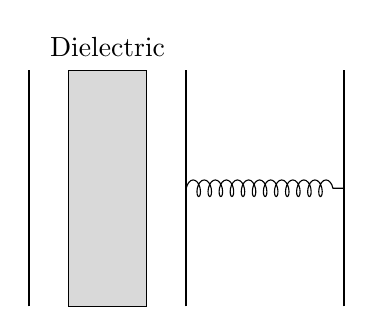
\begin{tikzpicture}[scale=1]

% Capacitor plates
\draw[thick] (0,0) -- (0,3);
\draw[thick] (2,0) -- (2,3);

% Dielectric slab
\draw[fill=gray!30] (0.5,0) rectangle (1.5,3);
\node at (1,3.3) {Dielectric};

% Spring
\draw[decorate,decoration={coil,aspect=0.5,segment length=4pt,amplitude=3pt}]
(2,1.5) -- (4,1.5);

% Wall
\draw[thick] (4,0) -- (4,3);

\end{tikzpicture}
\end{center}

\begin{enumerate}
\item[(A)] $\sqrt{\dfrac{k}{m} + \dfrac{Q^2}{2mC^2}\dv[2]{C}{x}}$
\item[(B)] $\sqrt{\dfrac{k}{m} - \dfrac{Q^2}{2mC^2}\dv[2]{C}{x}}$
\item[(C)] $\sqrt{\dfrac{k}{m} + \dfrac{Q^2}{mC^2}\dv[2]{C}{x}}$
\item[(D)] $\sqrt{\dfrac{k}{m} - \dfrac{Q^2}{mC^2}\dv[2]{C}{x}}$
\end{enumerate}

%%%%%%%%%%%%%%%%%%%%%%%%%%%%%%%%%%%%%%%%%%%%%%%%%%%%%%%%%%%%
\textbf{Q9. Rolling Cylinder in Upward Accelerating Lift with Curved Constraint}


Inside a lift accelerating upward with acceleration $a$, a solid cylinder of radius $R$ rests in a smooth circular groove of large radius such that its center performs small angular oscillations about the lowest point. Rolling without slipping occurs.

Using effective gravity $g+a$ and rotational kinetic energy contribution, determine the small oscillation frequency.

\begin{center}
\begin{tikzpicture}[scale=1]

% Groove centered at origin
\draw[thick] (-3,0) arc (180:360:3);

% Cylinder radius
\def\R{0.8}

% Cylinder center at lowest point inside groove
\draw[thick] (0,3-\R) circle (\R);
\node at (0,3-\R) {$R$};

% Lift acceleration arrow
\draw[->,thick] (-4,1) -- (-4,3);
\node at (-4,3.3) {$a$};

\end{tikzpicture}
\end{center}

\begin{enumerate}
\item[(A)] $\sqrt{\dfrac{2(g+a)}{3R}}$
\item[(B)] $\sqrt{\dfrac{3(g+a)}{2R}}$
\item[(C)] $\sqrt{\dfrac{(g+a)}{R}}$
\item[(D)] $\sqrt{\dfrac{4(g+a)}{3R}}$
\end{enumerate}

%%%%%%%%%%%%%%%%%%%%%%%%%%%%%%%%%%%%%%%%%%%%%%%%%%%%%%%%%%%%
\textbf{Q10. Charged Particle in Crossed Fields with Gravity}

A particle of charge $q$ and mass $m$ moves in uniform electric field $E$ (horizontal), magnetic field $B$ (into page), and gravitational field $g$ downward. Determine the steady horizontal drift velocity when vertical acceleration is zero.

\begin{enumerate}
\item[(A)] $qE = qv_dB$
\item[(B)] $qE + mg = qv_dB$
\item[(C)] $qE = qv_dB + mg$
\item[(D)] $qE - mg = qv_dB$
\end{enumerate}

%%%%%%%%%%%%%%%%%%%%%%%%%%%%%%%%%%%%%%%%%%%%%%%%%%%%%%%%%%%%
\textbf{Q11. Three-Spring Symmetric Mode System}



Two identical masses $m$ are connected by a spring of constant $k$, and each mass is attached to a fixed wall by identical springs $k$. The system oscillates in one dimension without friction.

Determine the angular frequency of symmetric mode using normal coordinate method.

\begin{center}
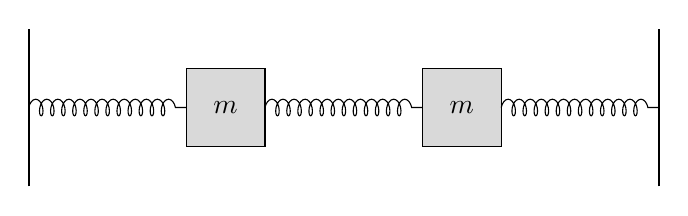
\begin{tikzpicture}[scale=1]

% Left wall
\draw[thick] (-1,0) -- (-1,2);

% Right wall
\draw[thick] (7,0) -- (7,2);

% Left spring
\draw[decorate,decoration={coil,aspect=0.5,segment length=4pt,amplitude=3pt}]
(-1,1) -- (1,1);

% First mass
\draw[fill=gray!30] (1,0.5) rectangle (2,1.5);
\node at (1.5,1) {$m$};

% Middle spring
\draw[decorate,decoration={coil,aspect=0.5,segment length=4pt,amplitude=3pt}]
(2,1) -- (4,1);

% Second mass
\draw[fill=gray!30] (4,0.5) rectangle (5,1.5);
\node at (4.5,1) {$m$};

% Right spring
\draw[decorate,decoration={coil,aspect=0.5,segment length=4pt,amplitude=3pt}]
(5,1) -- (7,1);

\end{tikzpicture}
\end{center}

\begin{enumerate}
\item[(A)] $\sqrt{\dfrac{2k}{m}}$
\item[(B)] $\sqrt{\dfrac{3k}{m}}$
\item[(C)] $\sqrt{\dfrac{k}{m}}$
\item[(D)] $\sqrt{\dfrac{4k}{m}}$
\end{enumerate}

%%%%%%%%%%%%%%%%%%%%%%%%%%%%%%%%%%%%%%%%%%%%%%%%%%%%%%%%%%%%
\textbf{Q12. Particle in Rotating Frame Gravitational Effective Potential}

A particle in rotating frame experiences effective potential
\[
U = -\frac{GMm}{r} + \frac12 m\omega^2 r^2.
\]
Determine the stable circular radius by minimizing total effective potential.

\begin{enumerate}
\item[(A)] $\left(\dfrac{GM}{\omega^2}\right)^{1/3}$
\item[(B)] $\left(\dfrac{2GM}{\omega^2}\right)^{1/3}$
\item[(C)] $\left(\dfrac{GM}{2\omega^2}\right)^{1/3}$
\item[(D)] $\left(\dfrac{3GM}{\omega^2}\right)^{1/3}$
\end{enumerate}

%%%%%%%%%%%%%%%%%%%%%%%%%%%%%%%%%%%%%%%%%%%%%%%%%%%%%%%%%%%%
\textbf{Q13. Conducting Loop Entering Magnetic Field Region}



A square conducting loop of side $a$, mass $m$, and resistance $R$ enters a region of uniform magnetic field $B$ with velocity $v$. Immediately after entry, induced current produces magnetic braking force.

Using Faraday’s law and instantaneous current approximation, determine initial deceleration magnitude.

\begin{center}
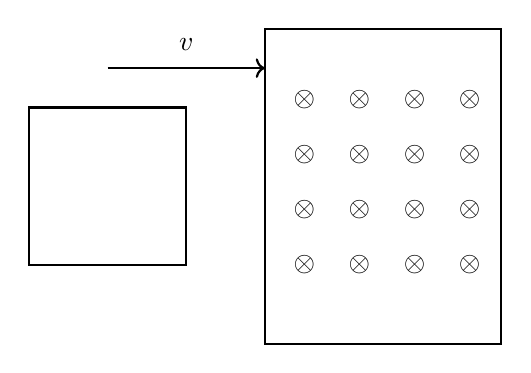
\begin{tikzpicture}[scale=1]

% Magnetic region
\draw[thick] (3,-1) rectangle (6,3);
\foreach \x in {3.5,4.2,4.9,5.6}
  \foreach \y in {0,0.7,1.4,2.1}
    \node at (\x,\y) {$\otimes$};

% Loop
\draw[thick] (0,0) rectangle (2,2);

% Velocity arrow
\draw[->,thick] (1,2.5) -- (3,2.5);
\node at (2,2.8) {$v$};

\end{tikzpicture}
\end{center}

\begin{enumerate}
\item[(A)] $\dfrac{B^2 a^2 v}{mR}$
\item[(B)] $\dfrac{B^2 a^4 v}{mR}$
\item[(C)] $\dfrac{2B^2 a^2 v}{mR}$
\item[(D)] $\dfrac{B^2 a^2 v}{2mR}$
\end{enumerate}

%%%%%%%%%%%%%%%%%%%%%%%%%%%%%%%%%%%%%%%%%%%%%%%%%%%%%%%%%%%%
\textbf{Q14. LC Circuit with Mechanical Modulation of Capacitance}

An LC oscillator has inductance $L$ and capacitance $C$. If plate separation changes slightly causing a small change $\Delta C$, determine the first-order fractional shift in oscillation frequency $\omega = 1/\sqrt{LC}$.

\begin{enumerate}
\item[(A)] $-\dfrac12 \dfrac{\Delta C}{C}$
\item[(B)] $-\dfrac{\Delta C}{C}$
\item[(C)] $\dfrac12 \dfrac{\Delta C}{C}$
\item[(D)] $\dfrac{\Delta C}{C}$
\end{enumerate}

%%%%%%%%%%%%%%%%%%%%%%%%%%%%%%%%%%%%%%%%%%%%%%%%%%%%%%%%%%%%
\textbf{Q15. Circular Motion Under Combined Gravity and Magnetic Force}


A charged particle of mass $m$ and charge $q$ moves in a circular orbit of radius $r$ around a massive body of mass $M$. A uniform magnetic field $B$ is perpendicular to orbital plane. Depending on direction of motion, magnetic force may add to or oppose gravitational centripetal requirement.

Determine the correct circular motion condition.

\begin{center}
\begin{tikzpicture}[scale=1]

% Central mass
\fill (0,0) circle (4pt);
\node[below] at (0,0) {$M$};

% Orbit
\draw[dashed] (0,0) circle (3);

% Particle
\fill (3,0) circle (2pt);
\node[right] at (3,0) {$m,q$};

% Velocity
\draw[->] (3,0) -- (3,1);
\node at (3.3,0.7) {$v$};

% Magnetic field symbol
\node at (-3,3) {$\otimes B$};

\end{tikzpicture}
\end{center}

\begin{enumerate}
\item[(A)] $\dfrac{mv^2}{r} = \dfrac{GMm}{r^2} + qvB$
\item[(B)] $\dfrac{mv^2}{r} = \dfrac{GMm}{r^2} - qvB$
\item[(C)] $\dfrac{mv^2}{r} = \dfrac{GMm}{r^2} + \dfrac{qvB}{2}$
\item[(D)] $\dfrac{mv^2}{r} = \dfrac{GMm}{r^2} - \dfrac{qvB}{2}$
\end{enumerate}

\end{document}